% $Header: /cvsroot/latex-beamer/latex-beamer/solutions/conference-talks/conference-ornate-20min.en.tex,v 1.6 2004/10/07 20:53:08 tantau Exp $

\documentclass{article}
%\documentclass{beamer}
%\documentclass[t,handout]{beamer} %use this header to print slides

% This file is a solution template for:

% - Talk at a conference/colloquium.
% - Talk length is about 20min.
% - Style is ornate.
\usepackage{beamerarticle}
\usepackage{multimedia}
%\usepackage{enumerate}
% Copyright 2004 by Till Tantau <tantau@users.sourceforge.net>.
%
% In principle, this file can be redistributed and/or modified under
% the terms of the GNU Public License, version 2.
%
% However, this file is supposed to be a template to be modified
% for your own needs. For this reason, if you use this file as a
% template and not specifically distribute it as part of a another
% package/program, I grant the extra permission to freely copy and
% modify this file as you see fit and even to delete this copyright
% notice. 


\mode<presentation>
{
  \usetheme{Frankfurt}%{Darmstadt}%default Warsaw Bergen Madrid Frankfurt Berlin Goettingen

  % or ...

  \setbeamercovered{transparent}
  % or whatever (possibly just delete it)
}

\usecolortheme{seahorse}%seagull seahorse default whale
\usecolortheme{rose}
\usepackage[english]{babel}
% or whatever

\usepackage[latin1]{inputenc}
% or whatever
\usepackage{pstricks,pst-node,pst-text,pst-3d}

\usepackage{colortbl}
\usepackage{times}
\usepackage[T1]{fontenc}
% Or whatever. Note that the encoding and the font should match. If T1
% does not look nice, try deleting the line with the fontenc.


\title[Beamer By Example] % (optional, use only with long paper titles)
{Beamer By Example}

\subtitle
{Subtitle: Frankfurt Theme}

\author[dfg] % (optional, use only with lots of authors)
{Willie Dewit~\inst{1} \and Jessie May~\inst{2} \and David Griffiths~\inst{3}}
% - Give the names in the same order as the appear in the paper.
% - Use the \inst{?} command only if the authors have different
%   affiliation.

\institute[Universities of Somewhere and Elsewhere] % (optional, but mostly needed)
{
  \inst{1}%
  Department of Mathematics\\
  University of Somewhere
  \and
  \inst{2}%
  Scottish Institute for Higher \TeX nology
  \and
  \inst{3}%
  University of Dundee}
% - Use the \inst command only if there are several affiliations.
% - Keep it simple, no one is interested in your street address.

\date[CTP 2007] % (optional, should be abbreviation of conference name)
{Conference on Tasteful Presentations, 2007}
% - Either use conference name or its abbreviation.
% - Not really informative to the audience, more for people (including
%   yourself) who are reading the slides online

%\subject{Theoretical Computer Science}
% This is only inserted into the PDF information catalog. Can be left
% out. 



% If you have a file called "university-logo-filename.xxx", where xxx
% is a graphic format that can be processed by latex or pdflatex,
% resp., then you can add a logo as follows:

\usepackage{pgfpages}
%\pgfpagelayout{8 on 1}{a4paper,border shrink=5mm}

\pgfdeclareimage[height=0.5cm]{university-logo}{univlogo}
 \logo{\pgfuseimage{university-logo}}



% Delete this, if you do not want the table of contents to pop up at
% the beginning of each subsection:
\AtBeginSubsection[]
{
  \begin{frame}<beamer>
    \frametitle{Outline}
    \tableofcontents[currentsection,currentsubsection]
  \end{frame}
}


% If you wish to uncover everything in a step-wise fashion, uncomment
% the following command: 

%\beamerdefaultoverlayspecification{<+->}

% define some basic colours - already defined if pstricks is used
\setbeamercolor{blue}{fg=blue!90}
%  \newcommand{\blue}[1]{\usebeamercolor[fg]{blue}#1}
\setbeamercolor{red}{fg=red!80,bg=yellow}
%  \newcommand{\red}[1]{\usebeamercolor[fg]{red}#1}
\setbeamercolor{black}{fg=black!99}
%  \newcommand{\black}[1]{\usebeamercolor[fg]{black}#1}
\setbeamercolor{green}{fg=green!80}
 % \newcommand{\green}[1]{\usebeamercolor[fg]{green}#1}

\newcommand{\bs}{\ensuremath{\backslash}}

\begin{document}
\maketitle
\begin{frame}
  \titlepage
\end{frame}

\begin{frame}
  \frametitle{Outline}
  \tableofcontents[pausesections]
  % You might wish to add the option [pausesections]
\end{frame}


% Structuring a talk is a difficult task and the following structure
% may not be suitable. Here are some rules that apply for this
% solution: 

% - Exactly two or three sections (other than the summary).
% - At *most* three subsections per section.
% - Talk about 30s to 2min per frame. So there should be between about
%   15 and 30 frames, all told.

% - A conference audience is likely to know very little of what you
%   are going to talk about. So *simplify*!
% - In a 20min talk, getting the main ideas across is hard
%   enough. Leave out details, even if it means being less precise than
%   you think necessary.
% - If you omit details that are vital to the proof/implementation,
%   just say so once. Everybody will be happy with that.
\section{Structure}
\subsection{Features}
\begin{frame}
\frametitle{Beamer}
\framesubtitle{Features}
Written by Till Tantau while completing his PhD.
\begin{itemize}
\item Process with either \texttt{pdflatex} or \texttt{latex+dvips}\pause
\item Standard \LaTeX\ commands still work\pause
\item \texttt{tableofcontents} works \pause
\item Overlays \&  dynamic effects easily created\pause
\item Easy navigation through sections \&  subsections\pause
\item Many templates and examples included in package\pause
\item \texttt{article } style can be used to produce notes
\end{itemize}
\end{frame}

\subsection{Basics}
\begin{frame}[fragile]
  \frametitle{Sample Code}
\verb+\documentclass{beamer}+
  
\verb+\usetheme{Frankfurt}+

  Use \verb+\section{..}+  and \verb+\subsection{..}+ to
create items for the Table of Contents

\alert<1>{The code for a frame is ...}
\begin{verbatim}
  \subsection{Basics}
  \begin{frame}
    \frametitle{Sample Code}
          Frame content
          .
  \end{frame}
\end{verbatim}
\end{frame}
%%%%%%%%%%%%%%%%%%%%%%%%%%%%%%%%%%%%%%%%
%
%\begin{frame}[fragile]
%  \frametitle{Outline--Code}
%The next lines of code are:
%\begin{verbatim}
%   \section{Lists}
%   \subsection{Uncovering Text}
%   \begin{frame}
%    \frametitle{..title..}
%    \begin{uncoverenv}<2->
%       \alert<2>{Then the next frame ...}
%    \end{uncoverenv}
%   \end{frame}
%\end{verbatim}
%\begin{uncoverenv}<2->
%\alert<2>{The Table of Contents appears before each new section unless
%switched off}
%\end{uncoverenv}
%\end{frame}

\subsection{Colour}

\begin{frame}[fragile]
  \frametitle{Colouring Text}
This a 2--stage process
\begin{itemize}
\item {\red Define} {\green the} {\blue colour}

\setbeamercolor{blue}{fg=blue!50}
\verb+\setbeamercolor{blue}{fg=blue!50}+\pause
\item Use the colour

\verb+{\usebeamercolor[fg]{blue} Some blue text}+

	{\usebeamercolor[fg]{blue} Some blue text}
\pause
\item or
{\small\verb+\newcommand{\green}[1]{\usebeamercolor[fg]{green}#1}+}

\verb+\green{some green text}+....\green{some green text}

\end{itemize}

\alert<4>{\texttt{\bs alert<4>\{Colours predefined in \textsc{pstricks}\}}}%\usebeamercolor[fg]{normal text}\{Colours predefined in \textsc{pstricks}\}}
\end{frame}


\section{Lists}

\subsection{Uncovering Text}
%%%%%%%%%%%%%%%%%%%%%%%%%%%%%%%%%%%%%%%%
\begin{frame}[fragile]
  \frametitle{Uncovering Text}
  \framesubtitle{Subtitle: A Short Example}

  \begin{itemize}
  \item
    Use \texttt{itemize} a lot--with \verb+\pause+\pause
  \item
    Use very short sentences or short phrases.
  \end{itemize}

  \begin{uncoverenv}<2>
  \begin{verbatim}
  \begin{itemize}
  \item
    Use \texttt{itemize} a lot--with \pause
  \item
    Use very short sentences or short phrases.
  \end{itemize}
  \end{verbatim}
  \end{uncoverenv}
\end{frame}
%%%%%%%%%%%%%%%%%%%%%%%%%%%%%%%%%%%%%%%%

\begin{frame}[fragile]
  \frametitle{Uncovering Text}
  \framesubtitle{Subtitle: A Longer Example}

  You can create overlays\dots
  \begin{itemize}
  \item using the \verb+\pause+ command:
    \begin{itemize}
    \item
      First item. (\verb+\pause+)
      \pause
    \item    
      Second item.
    \end{itemize}
  \item
    using overlay specifications: 
    \begin{itemize}
    \item<3->
      First item. (\verb+\item<3->+)
    \item<4>
      Second item.(\verb+\item<4>+)
    \end{itemize}
  \item
    using the general \verb+\uncover+ command:

    (\verb+\uncover<5->{\item First item...}+)
    \begin{itemize}
      \uncover<5->{\item First item. } 
      \uncover<6->{\item Second item. } 
    \end{itemize}
  \end{itemize}
\end{frame}

% \begin{frame}
%   \frametitle{Make Titles Informative.}
% Subsequent work
% \end{frame}

 
\begin{frame}[fragile]
\frametitle{Uncover \& alert}
\begin{columns}[c]
\begin{column}{.3\textwidth}
\begin{itemize}[<+-| alert@+>]
   \item Apple
   \item Peach
   \item Plum
   \item Orange
\end{itemize}
\end{column}
\begin{column}{.7\textwidth}
\begin{verbatim}
\begin{itemize}[<+-| alert@+>]
   \item Apple
   \item Peach
   \item Plum
   \item Orange
\end{itemize}
\end{verbatim}
\end{column}

\end{columns}
\end{frame}

%\subsection{Revelations}

%%%%%%%%%%%%%%%%%%%%%%%%%%%%%%%%%%%%%%%%
\begin{frame}[fragile]
  \frametitle{Uncovering Equations}

\begin{align*}
A &= \uncover<2->{B}\\
\uncover<3->{&=C\\}
\uncover<4->{&=D\\}
\end{align*}

\begin{uncoverenv}<4>
	\begin{verbatim}
\begin{align*}
A &=  \uncover<2->{B}\\
\uncover<2->{&=C\\}
\uncover<3->{&=D\\}
\end{align*}

	\end{verbatim}
  \end{uncoverenv}
\end{frame}

\begin{frame}
\frametitle{An example of replacement}
This uses five overlays, each separate equations\dots 
\alt<1>{
\[
\frac{\mathrm{d}}{\mathrm{d}x}\frac{x+3}{(x-1)^{2}}=\phantom{
\frac{(x-1)^{2}- (x+3)2 (x-1)}{(x-1)^{4}}}
\]}%
{%
\[
\frac{\mathrm{d}}{\mathrm{d}x}\frac{x+3}{(x-1)^{2}}
=
\frac{(x-1)^{2}- 2(x+3) (x-1)}{(x-1)^{4}}
\]}
\visible<3->{
\[
\phantom{\frac{\mathrm{d}}{\mathrm{d}x}\frac{x+3}{(x-1)^{2}}}=
\frac{\red(x-1)\black^{2}- 2(x+3) \red(x-1)\black}{\red(x-1)\black^{4}}
\]}
\visible<4->{
\[
\phantom{\frac{\mathrm{d}}{\mathrm{d}x}\frac{x+3}{(x-1)^{2}}}=
\frac{\red(x-1)\black ((x-1)- 2(x+3))}{\red(x-1)\black^{4}}
\]}
\visible<5->{
\[
\phantom{\frac{\mathrm{d}}{\mathrm{d}x}\frac{x+3}{(x-1)^{2}}}=
\frac{((x-1)- 2(x+3))}{(x-1)^{3}}=
-\frac{x+7}{(x-1)^{3}}
\]}
\uncover<2>{\bs {\blue{alt}} is used to replace the first line} \uncover<3>{and then \bs {\blue{visible}}, as opposed to \bs {\blue{uncover}}.} \alert<6>{Alignment not ideal.}
\end{frame}
%%%%%%%%%%%%%%%%%
\begin{frame}[fragile]
\frametitle{An example of \texttt{align} with replacement}
Three overlays, \dots 

\begin{align*}
left&=\alt<1>{\text{rhs 1}}{\text{alternate rhs}}\\
\visible<3->{&=\text{rhs 3}}
\end{align*}

\begin{verbatim}  
\begin{align*}
   left&=\alt<1>{rhs1}{\text{alternate rhs}}\\
  \visible<3->{&=rhs3}
\end{align*}
\end{verbatim}
\uncover<4->{Uses
\bs {\blue{alt}} and \bs {\blue{visible}}, as opposed to \bs {\blue{uncover}}.}
\uncover<5>{Alignment spoiled because alternative is longer than original.}
\end{frame}
%%%%%%%%%%%%%%%%%
\begin{frame}[fragile]
\frametitle{An example of \texttt{align} with replacement}
Use of  \bs{\blue{phantom}} to add invisible text to 3rd overlay to ensure correct alignment when \bs {\blue{alt}} string is longest\dots 

\begin{align*}
\text{left}&=\alt<1>{\text{rhs 1}}{\text{alternate rhs 2}}\\
\visible<3->{&=\text{rhs 3}\phantom{extra appended}}\\
\end{align*}

{\small\begin{verbatim}  
\begin{align*}
   \text{left}&=
        \alt<1>{\text{rhs 1}}{\text{alternate rhs 2}}\\
   \visible<3->
        {&=\text{rhs 3}\phantom{extra appended}}\\
\end{align*}
\end{verbatim}}
\end{frame}

%%%%%%%%%%%%%%%%%
\begin{frame}
\frametitle{The \texttt{align} environment with replacement}
 

\begin{align*}
\frac{\mathrm{d}}{\mathrm{d}x}\frac{x+3}{(x-1)^{2}}&=\alt<1>{}{
\frac{(x-1)^{2}- 2(x+3) (x-1)}{(x-1)^{4}}}{}\\
\visible<3->{&=\frac{\red(x-1)\black^{2}- 2(x+3) \red(x-1)\black}{\red(x-1)\black^{4}}}\\
\visible<4->{&=\frac{\red(x-1)\black ((x-1)- 2(x+3))}{\red(x-1)\black^{4}}}\\
\visible<5->{&=\frac{((x-1)- 2(x+3))}{(x-1)^{3}}=
-\frac{x+7}{(x-1)^{3}}
}\\
\end{align*}


\uncover<2->{\bs {\blue{alt}} replaces the first line} \uncover<3->{and then \bs {\blue{visible}}, as opposed to \bs {\blue{uncover}}}.
\uncover<5->{Alignment is fixed.}
\end{frame}

%%%%%%%%%%%%%%%%%%%%%%%%%%%%%%%%%%%%%%%%
\begin{frame}[fragile]
  \frametitle{Uncovering Rows}
\rowcolors[]{1}{blue!20}{red!10}
\begin{tabular}{l!{\vrule}cccc}
Class &	A &	 B &	 C &	 D\\\hline
X &	1 &	 2 &	3 &	4 \\\pause
Y &	 3 &	 4 &	 5 &	6 \\\pause
Z &     5 &	6 &	7 &	8
\end{tabular}
\smallskip

\setbeamercolor{blue text}{fg=blue!80}
  \begin{uncoverenv}<4->
  {\usebeamercolor[fg]{blue text} \verb+\usepackage{colortbl}+}
  \end{uncoverenv}

  \begin{uncoverenv}<5>
  \begin{verbatim}
\rowcolors[]{1}{blue!20}{red!10}
\begin{tabular}{l!{\vrule}cccc}\hline
Class &	A &	 B &	 C &	 D\\\hline
X &	1 &	 2 &	 3 &	 4 \\\pause
Y &	3 &	 4 &	 5 &	 6 \\\pause
Z &     5 & 	 6 &	 7 &	 8
\end{tabular}

  \end{verbatim}
  \end{uncoverenv}
\end{frame}
%%%%%%%%%%%%%%%%%%%%%%%%%%%%%%%%%%%%%%%%

\begin{frame}[fragile]
  \frametitle{Uncovering Columns}

\rowcolors[]{1}{blue!20}{red!10}
\begin{tabular}{l!{\vrule}c<{\onslide<2->}c<{\onslide<3>}c<{\onslide<4->}c<{\onslide<5->}c<{\onslide}c}
Class &	A &	 B &	 C &	 D\\
X &	1 &	 2 &	3 &	4\\
Y &	 3 &	 4 &	 5 &	6\\
Z &     5 &	6 &	7 &	8
\end{tabular}

  \begin{uncoverenv}<3->
  {{\begin{verbatim}
\begin{tabular}% 
  {l!{\vrule}c<{\onslide<2->}%
     c<{\onslide<3>}
     c<{\onslide<4->}c}
     ....
 \end{tabular}
  \end{verbatim}}}
  \end{uncoverenv}
\alert<4->{\texttt{\blue c<\{decl.\}} inserts decl. right after the entry for the column.}
\end{frame}
%%%%%%%%%%%%%%%%%%%%%%%%%%%%%%%%%%%%%%%%


\subsection{Theorems/Proofs}

\begin{frame}
  \frametitle{Theorem and Proof}
	\begin{theorem}
 There is no largest prime number 
\end{theorem}

\begin{proof}
\begin{itemize}
\item Suppose $p$ ... the largest prime\pause
\item Let $q$ be the product of the first $p$ numbers\pause
\item Then $q+1$ is not divisible by any of them\pause
\item Thus $q+1$ is a prime number larger than $p$.\pause
\end{itemize}

\end{proof}
\end{frame}
%%%%%%%%%%%%%%%%%%%%%%%%%%%%%%%%%%%%%%%%



\begin{frame}[fragile]
  \frametitle{Theorem and Proof-\blue{Code}}
\begin{verbatim}
\begin{theorem}
   There is no largest prime number 
\end{theorem}

\begin{proof}
\begin{itemize}
\item Suppose $p$ were the largest prime\pause
\item Let $q$ be ... first $p$ numbers\pause
\item Then $q+1$ is not divisible ...\pause
\item Thus $q+1$ is a prime ... $p$.\pause
\end{itemize}
\end{proof}
\end{verbatim}
\end{frame}

%%%%%%%%%%%%%%%%%%%%%%%%%%%%%%
\frame<1>[label=Cantor]
{\frametitle{Cantor's Theorem}
\begin{Theorem}
$\alpha <2^\alpha$ for all ordinals~$\alpha$.
\end{Theorem}
\begin{overprint}
\onslide<1>
\hyperlink{Cantor<2>}{\beamergotobutton{Proof details}}
\onslide<2->
% this is only shown in the appendix, where this frame is resumed.
\begin{proof}
As shown by Cantor...
\end{proof}
\hfill\hyperlink{Cantor<1>}{\beamerreturnbutton{Return}}
\end{overprint}
}

%%%%%%%%%%%%%%%%%%%%%%%%%%%%%%

\subsection{Handouts}

\begin{frame}[fragile]
  \frametitle{Printing slides for handouts}

With the header

%\begin{verbatim}
 {\blue{\bs documentclass[t,handout]\{beamer\}}}
%\end{verbatim}

\begin{enumerate}%[<+->][(i)]
\item the \texttt{\blue{t}} option specifies vertically aligned top frames
\item all piecewise defined slides are aggregated into one.

\item
\begin{verbatim}
\usepackage{enumerate}
...
\begin{enumerate}[<+->][(i)]
  \item the \texttt{\blue{t}} option specifies ....
  \item all piecewise defined ....
\end{enumerate}
\end{verbatim}
\end{enumerate}


\end{frame}

%%%%%%%%%%%%%%%%%%%%%%%%%%%%%%

\begin{frame}
   \frametitle{Printing as article class}
 
The header

 {\blue{\bs documentclass\{article\}}}
 
 and package
 
 {\blue{\bs usepackage\{beamerarticle\}}}
 
cause the material to be typeset as a ``normal'' article---all frame references are ignored.
 \end{frame}


%---------------------------------------------------------------------- SLIDE -
\section{Fancy Bits}
\subsection{Columns}
\begin{frame}[fragile]
\frametitle{Graphics \& Text  Side by Side}
\begin{columns}[b]
  \begin{column}{.25\textwidth}
       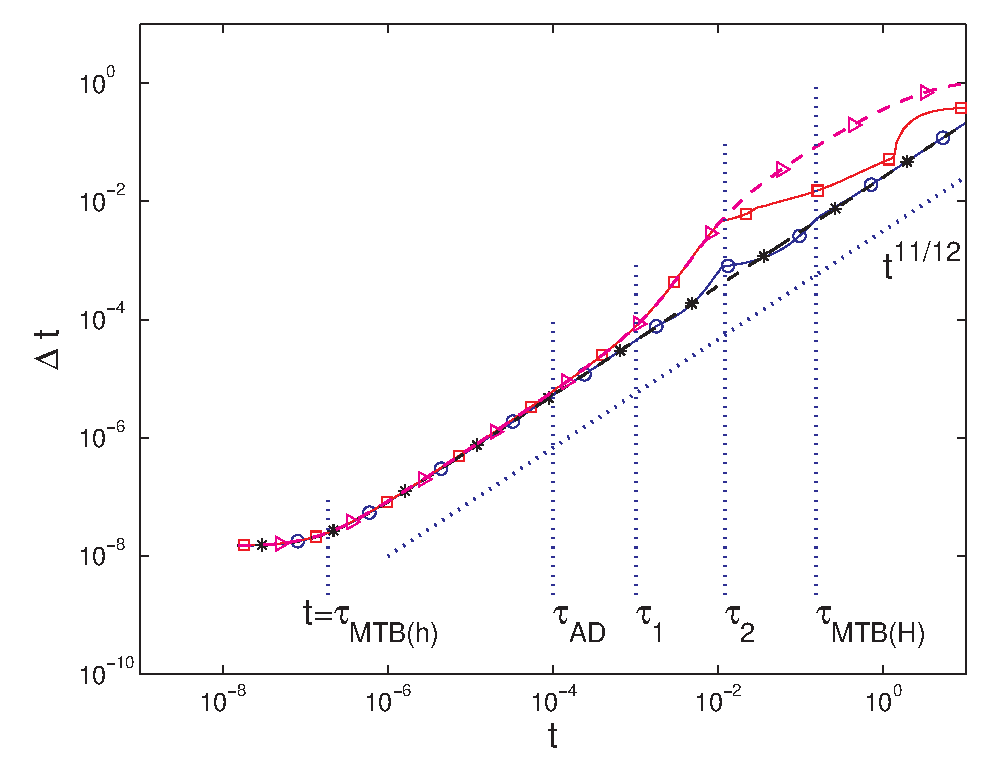
\includegraphics[width=1.1in]{advdiff_step-1.epsc}
  \end{column}
    \begin{column}{.75\textwidth}
    \begin{semiverbatim}
 \alert<1>{\\begin\{columns\}[b]}
  \alert<2>{\\begin\{column\}\{.25\\textwidth\}}
        \alert<3>{\\includegraphics[width=1.3in]%
             \{FILE.epsc\}}
  \alert<2>{\\end\{column\}}
   \alert<4>{\\begin\{column\}\{.75\\textwidth\}}
        \alert<5>{text column}
   \alert<4>{\\end\{column\}}
 \alert<1>{\\end\{columns\}}
    \end{semiverbatim}
    \uncover<6->{[We actually use \texttt{semiverbatim \& incremental alerts}.]}
      \end{column}
\end{columns}
\end{frame} 
\subsection{pstricks package} 
\begin{frame}[fragile]
\frametitle{Diagrams}
A small diagram with a few lines of \LaTeX.
\uncover<2->{
  At the 2nd overlay we can add a link from one to another using
\blue \rnode{start}{\textsc{PSTricks}}}%

\vspace{0.4cm}
{\tiny
\begin{equation*}
\setlength{\arraycolsep}{1cm}
\def\tX{\tilde{\tilde{X}}}
\begin{array}{cc}
        (X-A,N-A)\rnode{a}{} & \rnode{b}{}(\tX,a)\\[1.5cm]
        (X,N)\rnode{c}{} & \rnode{d}{}(\tX,N)\\[1.5cm]
\end{array}
\psset{nodesep=5pt,arrows=->}
\visible<2>{\nccurve[linecolor=red,angleA=270,angleB=300]{start}{c}}%
\ncline[linecolor=blue]{a}{b}\Aput{a}
\ncline[linecolor=blue]{a}{c}\Bput{r}
\ncline[linecolor=blue,linestyle=dashed]{c}{d}\Bput{b}
\ncline[linecolor=blue]{b}{d}\Bput{s}
\end{equation*}}
\vspace*{-.5in}\black
{\small\begin{verbatim}
  \blue \rnode{START}{\textsc{PSTricks}}
...
  \visible<2>{\nccurve%
      [linecolor=red,angleA=270,angleB=300]{START}{c}}
\end{verbatim}}
\end{frame}
%------------------------------------------------------------------------------

\begin{frame}
\frametitle{Householder formula}

The Householder formula below lets one compute $f(x_\ast)=0$ for an arbitrary $f$.
{%\scriptsize
\begin{equation}\label{Householder}
x_{k+1}\mapsto \Phi_n(x_k)=x_k+(n-1)
\frac{\left( \frac{1}{f(x_k)}\right)^{n{\displaystyle-}2}}
{\bigl(\frac{1}{f(x_k)}\bigr)^{n{\displaystyle-}1}}+
f(x_k)^{n+1}%
\alt<1>{\rnode{NA}{\pscirclebox[linecolor=red,linecolor=white]{\psi}}}
{\rnode{NA}{\pscirclebox[linecolor=red]{\psi}}}
\end{equation}}

\visible<2->{%
where $n\geq 2$ and \rnode{NB}{$\psi$} is an arbitrary function.}
\visible<2->{\nccurve[linecolor=red,angleA=90,angleB=270]{->}{NB}{NA}}

\visible<3>{
Formula~\eqref{Householder} gives an iteration of order $n$ converging
towards $x_{\ast}$ such that: $f(x_{\ast})=0$.}
\end{frame}
%---------------------------------------------------------------------- SLIDE -
\begin{frame}
\frametitle{Some \textsc{pstricks}}

Any practical use for this?

\begin{psclip}{\psellipse[linecolor=red]%
                (4.9,-1.7)(4,1.6)}
\begin{center}
\parbox{9cm}{%
{\green
ICMS--ICMS--ICMS--ICMS--ICMS--ICMS--ICMS--ICMS--ICMS--ICMS--ICMS--ICMS--ICMS--ICMS--ICMS--ICMS--%
ICMS--ICMS--ICMS--ICMS--ICMS--ICMS--ICMS--ICMS--ICMS--ICMS--ICMS--ICMS--ICMS--ICMS--ICMS--ICMS--%
ICMS--ICMS--ICMS--ICMS--ICMS--ICMS--ICMS--ICMS--ICMS--ICMS--ICMS--ICMS--ICMS--ICMS--ICMS--ICMS--%
ICMS--ICMS--ICMS--ICMS--ICMS--ICMS--ICMS--ICMS--ICMS--ICMS--ICMS--ICMS--ICMS--ICMS--ICMS--ICMS--%
ICMS--ICMS--ICMS--ICMS--ICMS--ICMS--ICMS--ICMS--ICMS--ICMS--ICMS--ICMS--ICMS--ICMS--ICMS--ICMS--%
ICMS--ICMS--ICMS--ICMS--ICMS--ICMS--ICMS--ICMS--ICMS--ICMS--ICMS--ICMS--ICMS--ICMS--ICMS--ICMS}}
\end{center}
\end{psclip}
\end{frame}
%---------------------------------------------------------------------- SLIDE -
\begin{frame}[fragile]
\frametitle{Some more \textsc{pstricks}}

or this ...
\begin{center}
\pstextpath{\psccurve[linestyle=none](.5,0)(3.5,1)(3.5,0)(.5,1)}%
{\blue ICMS--ICMS--ICMS--ICMS--ICMS--ICMS--ICMS--ICMS--ICMS--ICMS--ICM}
\end{center}
\begin{verbatim}
\pstextpath{\psccurve[linestyle=none]%
(.5,0)(3.5,1)(3.5,0)(.5,1)}%
{\blue ICMS--ICMS--ICMS--ICMS--ICMS--ICMS--%
ICMS--ICMS--ICMS--ICMS--ICM}
\end{verbatim}
\end{frame}

%------------------------------------------------------------------------------



%%%%%%%%%%%%%%%%%%%%%%%%%%%%%%%%%%
\subsection{Movies}

\begin{frame}[fragile]
  \frametitle{Including Movies}
\begin{verbatim}
\movie[width=3in,height=2in,showcontrols,poster]%
            {}{thank.avi}
\end{verbatim}

\mode<presentation>
\movie[width=2.5in, height=1.75in,showcontrols,poster]{}{thank.avi}
\mode
<all>
\medskip


Even though the movie is ``embedded'' in the \texttt{.tex} file, the \texttt{.avi} file must still reside in the same folder as the \texttt{pdf}  file.
\end{frame}


\section*{Summary}

\begin{frame}
  \frametitle<presentation>{Summary}

  % Keep the summary *very short*.
  \begin{itemize}
  \item
    The \alert{first main message} of your talk in one or two lines.\pause
  \item
    The \alert{second main message} of your talk in one or two lines.\pause
  \item
    Perhaps a \alert{third message}, but not more than that.\pause
  \end{itemize}
  
  % The following outlook is optional.
  \vskip0pt plus.5fill
  \begin{itemize}
  \item
    Outlook
    \begin{itemize}
    \item
      Something you haven't solved.
    \item
      Something else you haven't solved.
    \end{itemize}
  \end{itemize}
\end{frame}



% All of the following is optional and typically not needed. 
\appendix
\section<presentation>*{\appendixname}
\againframe<2>{Cantor}

\subsection<presentation>*{For Further Reading}

\begin{frame}[allowframebreaks]
  \frametitle<presentation>{For Further Reading}
    
  \begin{thebibliography}{10}
    
  \beamertemplatebookbibitems
  % Start with overview books.

  \bibitem{Author1990}
    A.~Author.
    \newblock {\em Handbook of Everything}.
    \newblock Some Press, 1990.
 
    
  \beamertemplatearticlebibitems
  % Followed by interesting articles. Keep the list short. 

  \bibitem{Someone2000}
    S.~Someone.
    \newblock On this and that.
    \newblock {\em Journal of This and That}, 2(1):50--100,
    2000.
    
    
    \bibitem{foo}
    D.F.~Griffiths
    \newblock Beamer By Example
    \newblock \texttt{http://www.maths.dundee.ac.uk/$\sim$dfg/talks.shtml}
  \end{thebibliography}
\end{frame}

\end{document}


